\begin{event}{International Conference on Formal Power Series and Algebraic Combinatorics}{FPSAC2019}{Ljubljana (SI),
  2019-07-01 to
  2019-07-05}{PS, FAU}{250}{2}{http://fpsac2019.fmf.uni-lj.si/}

\ODK participants: Nicolas M. Thi\'ery, Katja Ber\v{c}i\v{c}, Viviane
Pons.

\textbf{Event summary.} \href{http://fpsac.org}{FPSAC} -- Formal Power
Series and Algebraic Combinatorics -- is the major yearly
international conference on Algebraic; topics of presentations covered
all aspects of combinatorics and their relations with other parts of
mathematics, physics, computer science, and biology. This year's
edition took place in Ljubljana, Slovenia, from July 1st to 5th. About
250 mathematicians attended the event. One fourth of them also
attended the computational workshop Sage Days 105 organized on the
following week by ODK.

\textbf{\ODK implication.} N Thiéry is member of the permanent
committee of the conference since three years and has been leading an
effort to increase the strength of software demonstrations, as a way
to advertise and give back credit to the software development efforts
of its members. Indeed, this mathematical community has a long
tradition of using computer experimentation which plays a fundamental
role in the research. N. Thiéry chaired the software demonstration
sessions which held a record of six presentations, instead of a
handful for the previous years combined.

One presentation was delivered by K. Ber\v{c}i\v{c}, and presented an
early version of a website generator for mathematical databases, an
integral component of the \textsf{data.math\-hub.info} system
prototype (reported on in D6.10). All the materials for K.
Ber\v{c}i\v{c}'s software demonstration are available online:
\begin{itemize}
\item slides \url{http://fpsac2019.fmf.uni-lj.si/resources/Slides/202slides.pdf} and
\item extended abstract \url{http://fpsac2019.fmf.uni-lj.si/resources/Proceedings/202.pdf}
\end{itemize}

\ODK funded the participation of Nicolas M. Thiéry, K. Ber\v{c}i\v{c}
to the event (about 1100\euro). Coordinated efforts were undertaken
with the FPSAC organizers to encourage joint participation to both
events and optimize the funds used on both sides for supporting young
researcher.

\textbf{Results and impact.} The software demonstrations were well
received by the attendees. More than one half of the attendees were
present at the session, and a quick poll showed that most of them were
using computer experimentation on a regular basis, while a large
fraction was often writing code for their research.

All of the presentations used ODK components, and all the
demonstrations about computational software used Sage and were made
available online using the Binder service, with links from the
\href{http://fpsac2019.fmf.uni-lj.si/schedule/}{Schedule}.

There was a notable interest for the \textsf{data.math\-hub.info}
system prototype, which confirmed that there is a real need for such
infrastructure in the combinatorics community.

\begin{figure}[ht]
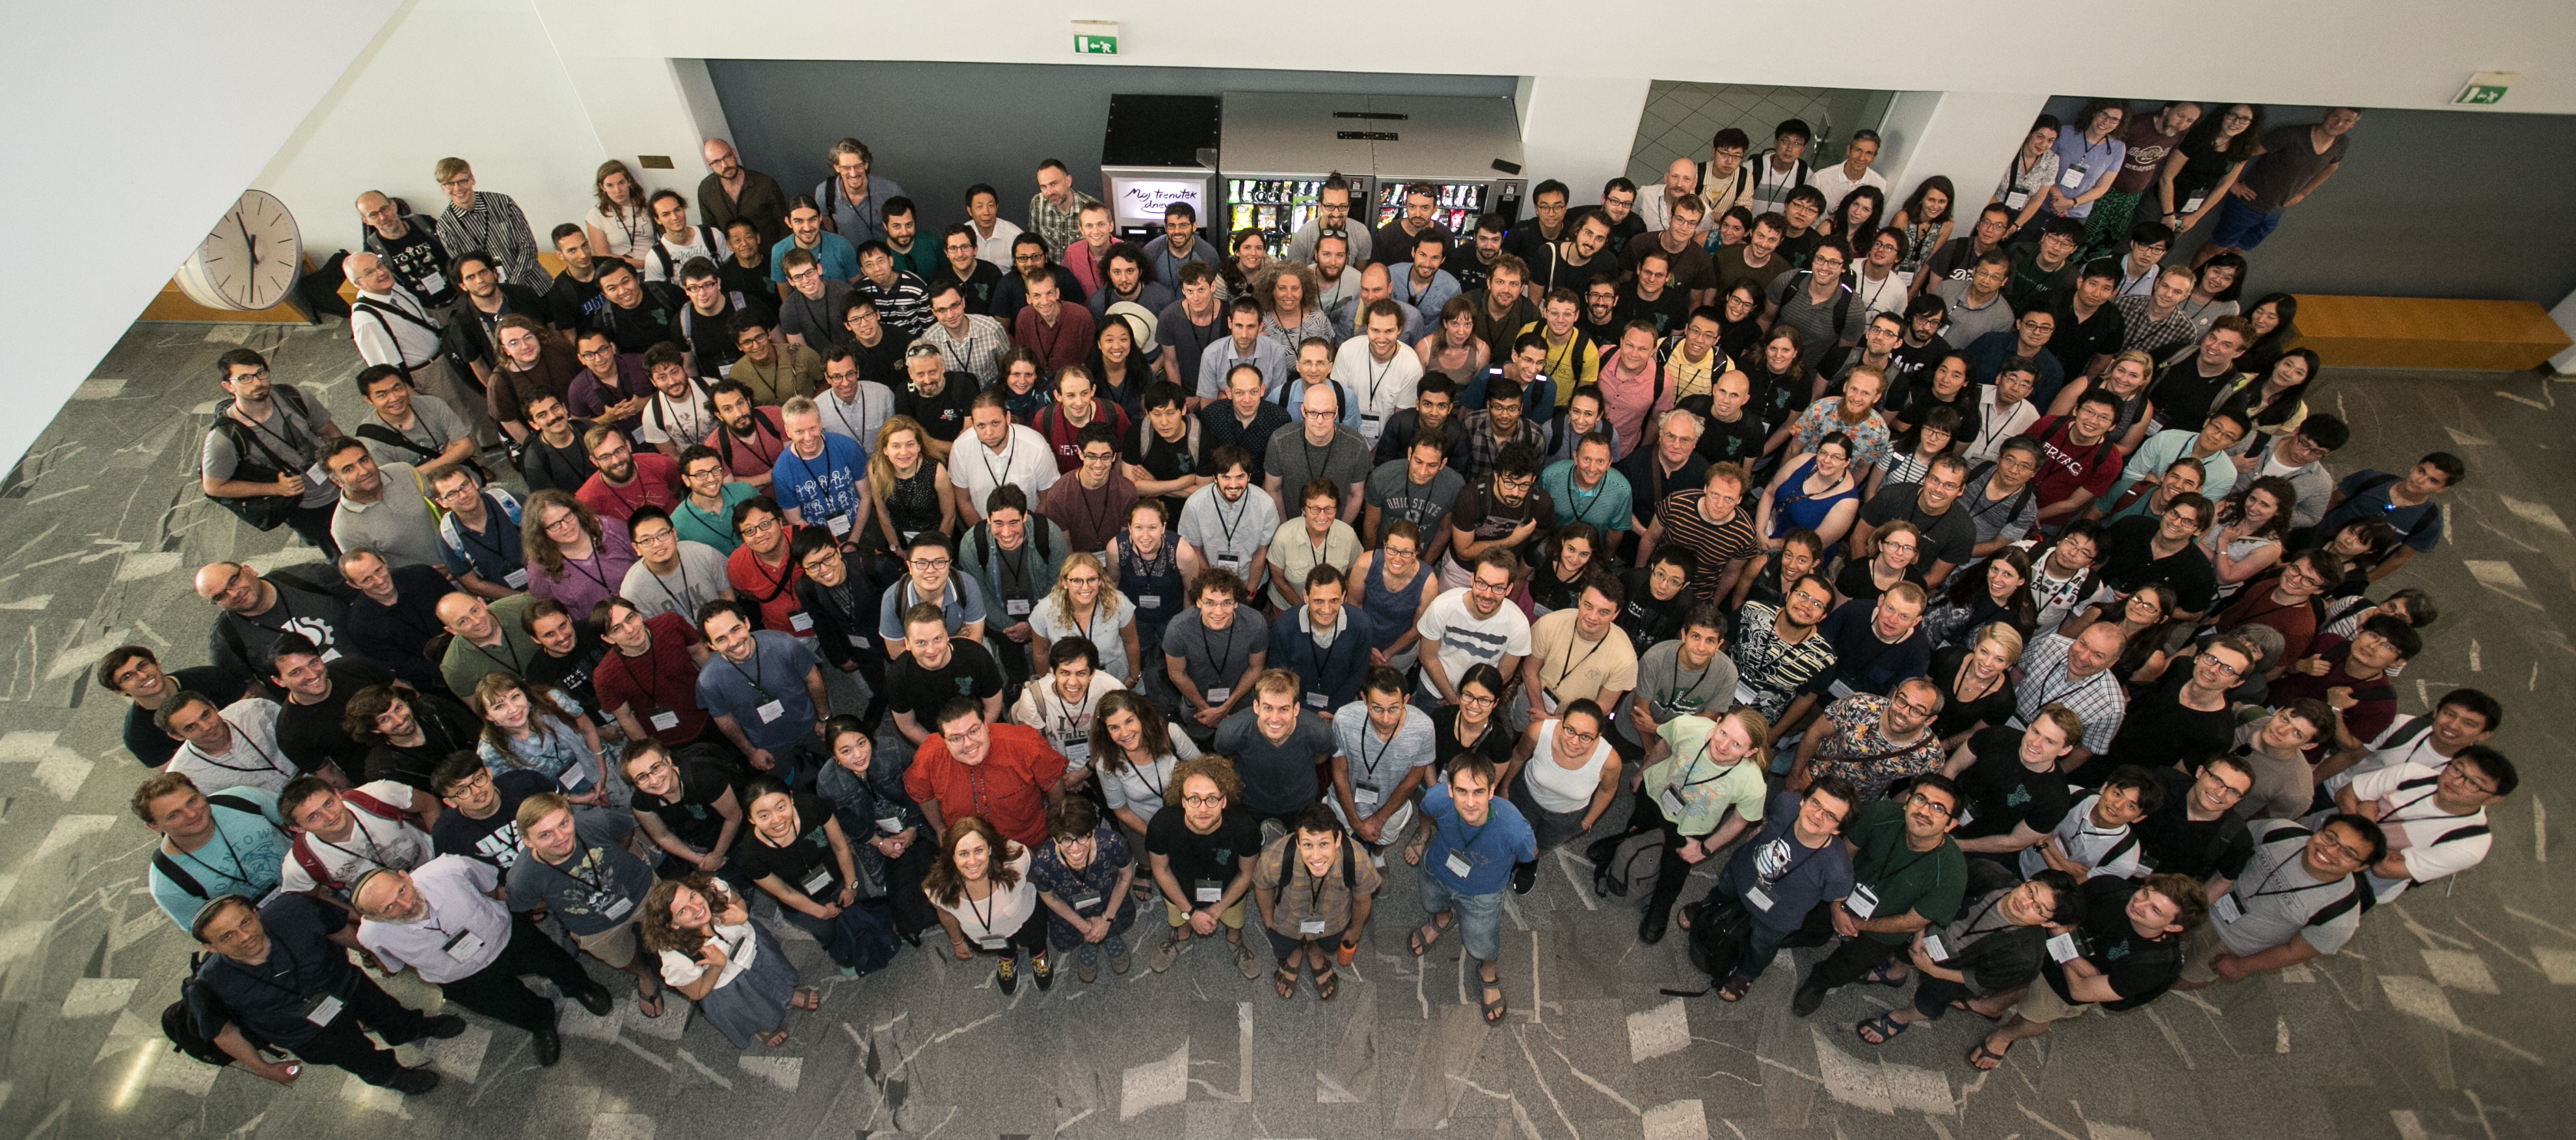
\includegraphics[scale=0.3]{FPSAC.jpg}
\caption*{International Conference on Formal Power Series and Algebraic Combinatorics, Ljubljana, Slovenia}
\end{figure}

\end{event}
